% Options for packages loaded elsewhere
% Options for packages loaded elsewhere
\PassOptionsToPackage{unicode}{hyperref}
\PassOptionsToPackage{hyphens}{url}
%
\documentclass[
  ignorenonframetext,
]{beamer}
\newif\ifbibliography
\usepackage{pgfpages}
\setbeamertemplate{caption}[numbered]
\setbeamertemplate{caption label separator}{: }
\setbeamercolor{caption name}{fg=normal text.fg}
\beamertemplatenavigationsymbolsempty
% remove section numbering
\setbeamertemplate{part page}{
  \centering
  \begin{beamercolorbox}[sep=16pt,center]{part title}
    \usebeamerfont{part title}\insertpart\par
  \end{beamercolorbox}
}
\setbeamertemplate{section page}{
  \centering
  \begin{beamercolorbox}[sep=12pt,center]{section title}
    \usebeamerfont{section title}\insertsection\par
  \end{beamercolorbox}
}
\setbeamertemplate{subsection page}{
  \centering
  \begin{beamercolorbox}[sep=8pt,center]{subsection title}
    \usebeamerfont{subsection title}\insertsubsection\par
  \end{beamercolorbox}
}
% Prevent slide breaks in the middle of a paragraph
\widowpenalties 1 10000
\raggedbottom
\AtBeginPart{
  \frame{\partpage}
}
\AtBeginSection{
  \ifbibliography
  \else
    \frame{\sectionpage}
  \fi
}
\AtBeginSubsection{
  \frame{\subsectionpage}
}
\usepackage{iftex}
\ifPDFTeX
  \usepackage[T1]{fontenc}
  \usepackage[utf8]{inputenc}
  \usepackage{textcomp} % provide euro and other symbols
\else % if luatex or xetex
  \usepackage{unicode-math} % this also loads fontspec
  \defaultfontfeatures{Scale=MatchLowercase}
  \defaultfontfeatures[\rmfamily]{Ligatures=TeX,Scale=1}
\fi
\usepackage{lmodern}

\usetheme[]{metropolis}
\ifPDFTeX\else
  % xetex/luatex font selection
\fi
% Use upquote if available, for straight quotes in verbatim environments
\IfFileExists{upquote.sty}{\usepackage{upquote}}{}
\IfFileExists{microtype.sty}{% use microtype if available
  \usepackage[]{microtype}
  \UseMicrotypeSet[protrusion]{basicmath} % disable protrusion for tt fonts
}{}
\makeatletter
\@ifundefined{KOMAClassName}{% if non-KOMA class
  \IfFileExists{parskip.sty}{%
    \usepackage{parskip}
  }{% else
    \setlength{\parindent}{0pt}
    \setlength{\parskip}{6pt plus 2pt minus 1pt}}
}{% if KOMA class
  \KOMAoptions{parskip=half}}
\makeatother


\usepackage{longtable,booktabs,array}
\usepackage{calc} % for calculating minipage widths
\usepackage{caption}
% Make caption package work with longtable
\makeatletter
\def\fnum@table{\tablename~\thetable}
\makeatother
\usepackage{graphicx}
\makeatletter
\newsavebox\pandoc@box
\newcommand*\pandocbounded[1]{% scales image to fit in text height/width
  \sbox\pandoc@box{#1}%
  \Gscale@div\@tempa{\textheight}{\dimexpr\ht\pandoc@box+\dp\pandoc@box\relax}%
  \Gscale@div\@tempb{\linewidth}{\wd\pandoc@box}%
  \ifdim\@tempb\p@<\@tempa\p@\let\@tempa\@tempb\fi% select the smaller of both
  \ifdim\@tempa\p@<\p@\scalebox{\@tempa}{\usebox\pandoc@box}%
  \else\usebox{\pandoc@box}%
  \fi%
}
% Set default figure placement to htbp
\def\fps@figure{htbp}
\makeatother





\setlength{\emergencystretch}{3em} % prevent overfull lines

\providecommand{\tightlist}{%
  \setlength{\itemsep}{0pt}\setlength{\parskip}{0pt}}



 


\setbeamerfont{title}{size=\large}
\usepackage{hyperref}
\setbeamertemplate{footline}[frame number]
\usepackage{tikz}
\usetikzlibrary{arrows.meta, positioning, shapes.geometric, fit, backgrounds, calc}
\usepackage{booktabs}
\usepackage{xcolor}
\definecolor{mblue}{RGB}{35,55,100}
\makeatletter
\@ifpackageloaded{caption}{}{\usepackage{caption}}
\AtBeginDocument{%
\ifdefined\contentsname
  \renewcommand*\contentsname{Table of contents}
\else
  \newcommand\contentsname{Table of contents}
\fi
\ifdefined\listfigurename
  \renewcommand*\listfigurename{List of Figures}
\else
  \newcommand\listfigurename{List of Figures}
\fi
\ifdefined\listtablename
  \renewcommand*\listtablename{List of Tables}
\else
  \newcommand\listtablename{List of Tables}
\fi
\ifdefined\figurename
  \renewcommand*\figurename{Figure}
\else
  \newcommand\figurename{Figure}
\fi
\ifdefined\tablename
  \renewcommand*\tablename{Table}
\else
  \newcommand\tablename{Table}
\fi
}
\@ifpackageloaded{float}{}{\usepackage{float}}
\floatstyle{ruled}
\@ifundefined{c@chapter}{\newfloat{codelisting}{h}{lop}}{\newfloat{codelisting}{h}{lop}[chapter]}
\floatname{codelisting}{Listing}
\newcommand*\listoflistings{\listof{codelisting}{List of Listings}}
\makeatother
\makeatletter
\makeatother
\makeatletter
\@ifpackageloaded{caption}{}{\usepackage{caption}}
\@ifpackageloaded{subcaption}{}{\usepackage{subcaption}}
\makeatother

\usepackage{bookmark}
\IfFileExists{xurl.sty}{\usepackage{xurl}}{} % add URL line breaks if available
\urlstyle{same}
\hypersetup{
  pdfauthor={Giorgio Arcara},
  hidelinks,
  pdfcreator={LaTeX via pandoc}}


\author{Giorgio Arcara}
\date{}

\begin{document}


\begin{frame}
\title{Metodologia della Ricerca Clinica\\
\vspace{0.5em}
{\normalsize 12. Studi correlazionali e inferenza causale}}
\author{Giorgio Arcara,\\ Università di Padova \\ IRCCS San Camillo, Venezia}
\titlegraphic{
\vspace*{7cm}
\includegraphics[scale=0.15]{Figures/LogoSanCamilloIRCCS_Unipd_alpha.png}
\hfill \includegraphics[scale=0.15]{Figures/CC_license_3_0.png}
}
\maketitle
\end{frame}

\section{3.1 Correlazione vs
Causalità}\label{correlazione-vs-causalituxe0}

\begin{frame}{La premessa}
\phantomsection\label{la-premessa}
Di base, nella scienza siamo sempre interessati a comprendere i
meccanismi causali.

Questo ci permette di capire come \textbf{intervenire} e produrre
\textbf{cambiamenti}.
\end{frame}

\begin{frame}{Il Problema Fondamentale}
\phantomsection\label{il-problema-fondamentale}
\small

La ricerca clinica osservazionale produce associazioni statistiche.

Ma un'associazione è sufficiente per fondare un intervento terapeutico?

Un associazione è sufficiente a stabilire una relazione causa-effetto?
\end{frame}

\begin{frame}{Correlation is not causation}
\phantomsection\label{correlation-is-not-causation}
\begin{center}
\includegraphics[width=0.8\linewidth,height=\textheight,keepaspectratio]{Figures/corrCause1.png}
\end{center}
\end{frame}

\begin{frame}{Il Problema}
\phantomsection\label{il-problema}
Spesso il problema della possibile confusione tra correlazione e causa è
banalizzato perché gli esempi per spiegarlo sono estremi (è facile
identificare la fallacia)

Numerose volte la fallacia viene comunque commessa nell'interprezione di
risultati, \emph{specie se la relazione causale è plausibile oppure se
relativa ad altre evidenze}.
\end{frame}

\begin{frame}{Esempi importanti}
\phantomsection\label{esempi-importanti}
\textbf{Esempio neuropsicologico}: In numerosi casi la correlazione tra
scolarità e diverse traiettorie di decadimento cognitivo è stata
interpretata con un ruolo ``protettivo''

\begin{center}
\includegraphics[width=0.7\linewidth,height=\textheight,keepaspectratio]{Figures/Fjell_2025.png}
\end{center}
\end{frame}

\begin{frame}{A contradictory result}
\phantomsection\label{a-contradictory-result}
\begin{center}
\includegraphics[width=0.8\linewidth,height=\textheight,keepaspectratio]{Figures/Fjell_results.png}
\end{center}
\end{frame}

\begin{frame}{Diverse relazioni, stesso effetto osservato}
\phantomsection\label{diverse-relazioni-stesso-effetto-osservato}
Se analizzassimo la relazione tra X e Y, troveremmo in questi tre casi
una forte correlazione (o ``predizione'' tramite regressione) tra X e Y.

\begin{center}
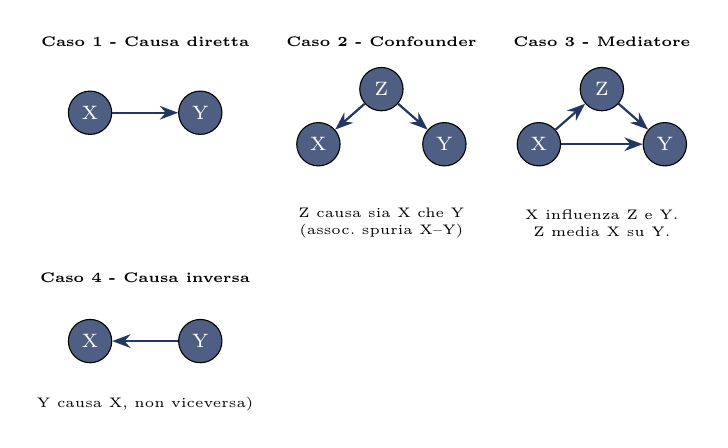
\begin{tikzpicture}[
  node/.style={circle,draw,fill=mblue!80,font=\scriptsize,
               minimum size=0.55cm,inner sep=1pt, text=white},
  arr/.style={-{Stealth},mblue,thick}
]

% ── Caso 1 ──────────────────────────────────────────────
\node[font=\tiny\bfseries] at (-5,3.2) {Caso 1 - Causa diretta};
\node[node] (X)  at (-5.7,2.3) {X};
\node[node] (Y)  at (-4.3,2.3) {Y};
\draw[arr] (X)--(Y);

% ── Caso 2 ──────────────────────────────────────────────
\node[font=\tiny\bfseries] at (-2,3.2) {Caso 2 - Confounder};
\node[node] (Z)  at (-2,2.6)  {Z};
\node[node] (X2) at (-2.8,1.9) {X};
\node[node] (Y2) at (-1.2,1.9) {Y};
\draw[arr] (Z)--(X2); \draw[arr] (Z)--(Y2);
\node[font=\tiny,align=center] at (-2,0.9) {Z causa sia X che Y\\(assoc.\ spuria X--Y)};

% ── Caso 3 ──────────────────────────────────────────────
\node[font=\tiny\bfseries] at (0.8,3.2) {Caso 3 - Mediatore};
\node[node] (Z2) at (0.8,2.6)  {Z};
\node[node] (X3) at (0.0,1.9)  {X};
\node[node] (Y3) at (1.6,1.9)  {Y};
\draw[arr] (X3)--(Z2); \draw[arr] (Z2)--(Y3);
\draw[arr] (X3)--(Y3);
\node[font=\tiny,align=center] at (0.8,0.9) {X influenza Z e Y.\\Z media X su Y.};

% ── Caso 4 ──────────────────────────────────────────────
\node[font=\tiny\bfseries] at (-5,0.2) {Caso 4 - Causa inversa};
\node[node] (X4) at (-5.7,-0.6) {X};
\node[node] (Y4) at (-4.3,-0.6) {Y};
\draw[arr] (Y4)--(X4);
\node[font=\tiny,align=center] at (-5,-1.4) {Y causa X, non viceversa)};

\end{tikzpicture}
\end{center}
\end{frame}

\begin{frame}{Problemi statistici nello studiare associazioni tra
variabili.}
\phantomsection\label{problemi-statistici-nello-studiare-associazioni-tra-variabili.}
\small

\begin{itemize}
\item
  \textbf{Collinearità}: se ho due variabili molto correlate, potrei non
  essere in grado di distinguere l'effetto e inserirle entrambe in un
  modello può creare distorsioni.
\item
  \textbf{Bias di selezione}: chi entra nel mio campione potrebbe non
  essere rappresentativo della popolazione (e.g.~\emph{self-selection}),
  il drop-out potrebbe essere legato ad una variabile rilevante,
  collider bias (vedi dopo).
\item
  \textbf{Direzione della relazione} difficilmente è facile capire la
  direzione della relazione (e.g.~ho alti punteggi cognitivi perché ho
  studiato molto oppure ho studiato molto perché ho alti score
  cognitivi?)
\item
  \textbf{Errore di misurazione} ricordiamoci sempre che c'è un errore
  di misurazione che potrebbe anche essere diverso tra i test
  utilizzati.
\end{itemize}
\end{frame}

\begin{frame}{Verso la causalità: I criteri di Bradford Hill}
\phantomsection\label{verso-la-causalituxe0-i-criteri-di-bradford-hill}
\textbf{Criteri di Bradford Hill} (1965): 9 criteri per valutare
l'evidenza di causalità in epidemiologia (forza, consistenza,
specificità, temporalità, dose-risposta, plausibilità biologica,
coerenza, esperimento, analogia).

\vspace{0.2em}

\tiny Bradford Hill (1965). The environment and disease: association or
causation? \emph{Proc R Soc Med} 58:295--300. Open Access:
\url{https://doi.org/10.1177/003591576505800503}
\end{frame}

\begin{frame}{Il Problema Fondamentale dell'Inferenza Causale}
\phantomsection\label{il-problema-fondamentale-dellinferenza-causale}
\small

Il \textbf{Fundamental Problem of Causal Inference} (Holland, 1986): non
possiamo mai osservare entrambi i \textbf{counterfactuals} per lo stesso
individuo nello stesso momento.

\vspace{0.4em}

\begin{center}
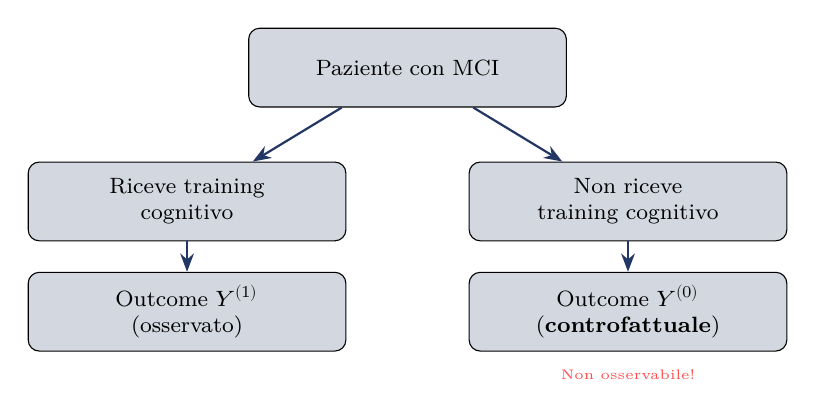
\begin{tikzpicture}[
  box/.style={draw,rounded corners,fill=mblue!20,text width=3.8cm,
              align=center,font=\footnotesize,minimum height=1cm},
  arr/.style={-{Stealth},mblue,thick}
]
\node[box] (paz) at (0,2.5) {Paziente con MCI};
\node[box] (t1)  at (-2.8,0.8) {Riceve training\\cognitivo};
\node[box] (t0)  at ( 2.8,0.8) {Non riceve\\training cognitivo};
\node[box] (y1)  at (-2.8,-0.6) {Outcome $Y^{(1)}$\\(osservato)};
\node[box] (y0)  at ( 2.8,-0.6) {Outcome $Y^{(0)}$\\(\textbf{controfattuale})};
\draw[arr] (paz)--(t1); \draw[arr] (paz)--(t0);
\draw[arr] (t1)--(y1);  \draw[arr] (t0)--(y0);
\node[font=\tiny,red!70] at (2.8,-1.4) {Non osservabile!};
\end{tikzpicture}
\end{center}

\small L'effetto causale individuale = \(Y^{(1)} - Y^{(0)}\). Ma
osserviamo solo uno dei due. La randomizzazione risolve il problema
\emph{in media} tra i gruppi.
\end{frame}

\section{3.2 DAG: Directed Acyclic
Graphs}\label{dag-directed-acyclic-graphs}

\begin{frame}{Cos'è un DAG?}
\phantomsection\label{cosuxe8-un-dag}
\small

Un \textbf{DAG} (Directed Acyclic Graph) è uno strumento per
rappresentare esplicitamente le \textbf{assunzioni causali} su un
sistema. Ogni freccia rappresenta un'ipotesi di relazione causale
diretta.

\vspace{0.3em}

\textbf{Componenti}: \footnotesize - \textbf{Nodi}: variabili (osservate
o latenti) - \textbf{Frecce}: relazioni causali dirette -
\textbf{Aciclico}: non ci sono cicli (A \(\to\) B \(\to\) A)

\vspace{0.3em}

\textbf{A cosa serve}:

\begin{itemize}\footnotesize
\item Identificare quali variabili controllare (e quali \emph{non} controllare)
\item Identificare confounders, mediatori, colliders
\item Valutare se un effetto causale è identificabile dai dati disponibili
\end{itemize}

\vspace{0.2em}

\tiny Textor et al.~(2016). Robust causal reasoning using DAGs.
\emph{Int J Epidemiol}.\textbackslash{} Strumento online: DAGitty ---
Open Access: \url{https://www.dagitty.net}
\end{frame}

\begin{frame}{Strutture Fondamentali nei DAG}
\phantomsection\label{strutture-fondamentali-nei-dag}
\begin{center}
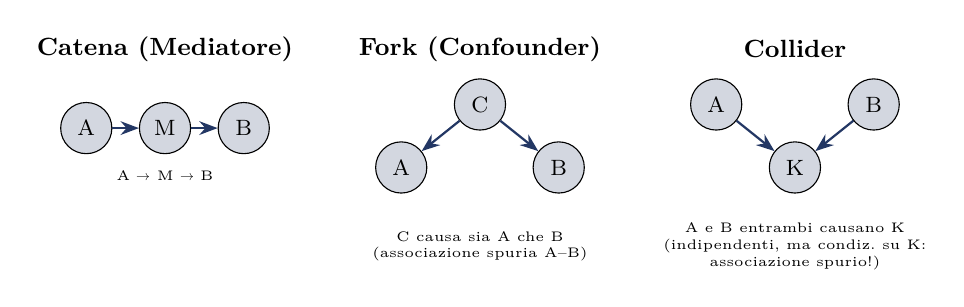
\begin{tikzpicture}[
  node/.style={circle,draw,fill=mblue!20,font=\footnotesize,
               minimum size=0.65cm,inner sep=1pt},
  arr/.style={-{Stealth},mblue,thick}
]
% Chain (mediator)
\node[font=\small\bfseries] at (-4,3.5) {Catena (Mediatore)};
\node[node] (A1) at (-5,2.5) {A};
\node[node] (M)  at (-4,2.5) {M};
\node[node] (B1) at (-3,2.5) {B};
\draw[arr] (A1)--(M); \draw[arr] (M)--(B1);
\node[font=\tiny] at (-4,1.9) {A $\to$ M $\to$ B};

% Fork (confounder)
\node[font=\small\bfseries] at (0,3.5) {Fork (Confounder)};
\node[node] (C)  at (0,2.8) {C};
\node[node] (A2) at (-1,2.0) {A};
\node[node] (B2) at (1,2.0)  {B};
\draw[arr] (C)--(A2); \draw[arr] (C)--(B2);
\node[font=\tiny,align=center] at (0,1) {C causa sia A che B\\(associazione spuria A--B)};

% Collider
\node[font=\small\bfseries] at (4,3.5) {Collider};
\node[node] (A3) at (3,2.8) {A};
\node[node] (B3) at (5,2.8) {B};
\node[node] (K)  at (4,2.0) {K};
\draw[arr] (A3)--(K); \draw[arr] (B3)--(K);
\node[font=\tiny,align=center] at (4,1) {A e B entrambi causano K\\(indipendenti, ma condiz.\ su K:\\associazione spurio!)};
\end{tikzpicture}
\end{center}
\end{frame}

\begin{frame}{Confounder: Esempio Neuropsicologico}
\phantomsection\label{confounder-esempio-neuropsicologico}
\begin{center}
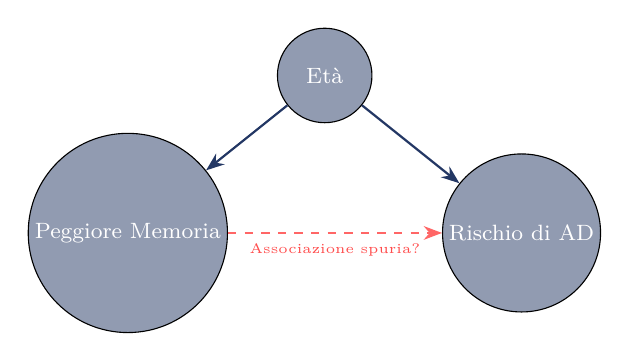
\begin{tikzpicture}[
  node/.style={circle,draw,fill=mblue!20,font=\footnotesize,
               minimum size=1.2cm,inner sep=2pt,align=center},
  obs/.style={circle,draw,fill=mblue!50,text=white,font=\footnotesize,
              minimum size=1.2cm,inner sep=2pt,align=center},
  arr/.style={-{Stealth},mblue,thick},
  spurious/.style={-{Stealth},red!60,dashed,thick}
]
\node[obs] (eta)  at (0,3)   {Età};
\node[obs] (dep)  at (-2.5,1) {Peggiore Memoria};
\node[obs] (cog)  at ( 2.5,1) {Rischio di AD};
\draw[arr]     (eta)--(dep);
\draw[arr]     (eta)--(cog);
\draw[spurious](dep)--(cog)
  node[midway,below,font=\tiny,red!70]{Associazione spuria?};
\end{tikzpicture}
\end{center}
\vspace{-0.3em}

\small L'età causa sia la depressione che il declino cognitivo. Se non
controlliamo per l'età, troviamo un'associazione depressione--cognizione
che potrebbe essere \textbf{totalmente} o \textbf{parzialmente} spuria.

\vspace{0.3em}

\textbf{Soluzione}: aggiungere l'età come covariata nella regressione
--- o meglio, costruire il DAG \emph{prima} di analizzare i dati.
\end{frame}

\begin{frame}{Collider: Un Errore Sottile}
\phantomsection\label{collider-un-errore-sottile}
\begin{center}
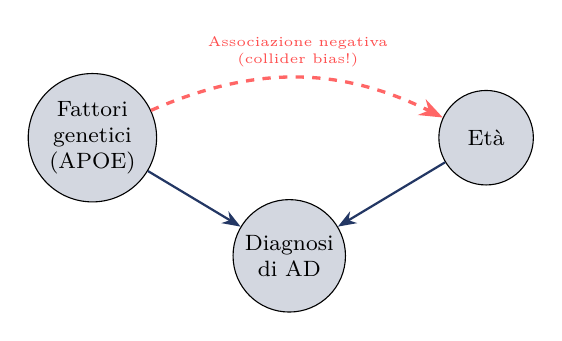
\begin{tikzpicture}[
  node/.style={circle,draw,fill=mblue!20,font=\footnotesize,
               minimum size=1.2cm,inner sep=2pt,align=center},
  arr/.style={-{Stealth},mblue,thick},
  spurious/.style={-{Stealth},red!60,dashed,very thick}
]
\node[node] (gen) at (-2.5,2) {Fattori\\genetici\\(APOE)};
\node[node] (tbi) at ( 2.5,2) {Età};
\node[node] (ad)  at (0,0.5)  {Diagnosi\\di AD};
\draw[arr] (gen)--(ad);
\draw[arr] (tbi)--(ad);
\draw[spurious] (gen) to[bend left=25] node[above,font=\tiny,red!70, align=center]{Associazione negativa\\(collider bias!)} (tbi);
\end{tikzpicture}
\end{center}
\vspace{-0.3em}

\small In un campione clinico (selezionato per avere AD), APOE ed Età
diventano \textbf{negativamente correlati} anche se nella popolazione
generale sono indipendenti.
\textbf{Condizionare su un collider apre un percorso spurio}.

\vspace{0.2em}

\footnotesize \textbf{Implicazione pratica}: studi condotti solo su
pazienti ospedalizzati o con una specifica diagnosi possono soffrire di
collider bias (noto anche come \emph{Berkson's bias}).
\end{frame}

\begin{frame}{Collider (covariata da non inserire)}
\phantomsection\label{collider-covariata-da-non-inserire}
\begin{center}
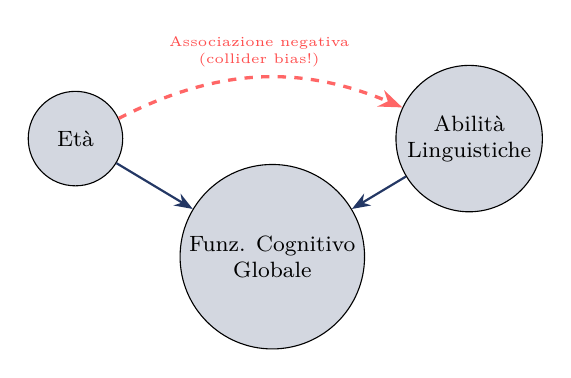
\begin{tikzpicture}[
  node/.style={circle,draw,fill=mblue!20,font=\footnotesize,
               minimum size=1.2cm,inner sep=2pt,align=center},
  arr/.style={-{Stealth},mblue,thick},
  spurious/.style={-{Stealth},red!60,dashed,very thick}
]
\node[node, align=center] (gen) at (-2.5,2) {Età};
\node[node] (tbi) at ( 2.5,2) {Abilità\\ Linguistiche};
\node[node] (ad)  at (0,0.5)  {Funz. Cognitivo\\ Globale};
\draw[arr] (gen)--(ad);
\draw[arr] (tbi)--(ad);
\draw[spurious] (gen) to[bend left=25] node[above,font=\tiny,red!70, align=center]{Associazione negativa\\(collider bias!)} (tbi);
\end{tikzpicture}
\end{center}
\vspace{-0.3em}

\small Controllando per un \textbf{collider} rischiamo di avere stime
distorte (es. inserendo una covariata in un modello di regressione)
\end{frame}

\begin{frame}{Mediatore: Non Sempre va Controllato}
\phantomsection\label{mediatore-non-sempre-va-controllato}
\begin{center}
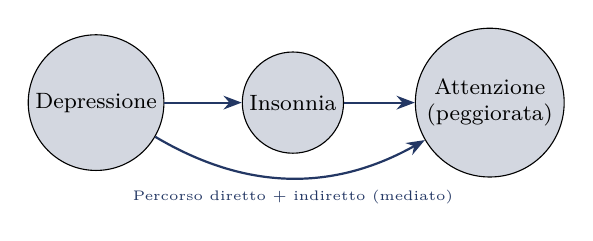
\begin{tikzpicture}[
  node/.style={circle,draw,fill=mblue!20,font=\footnotesize,
               minimum size=1.2cm,inner sep=2pt,align=center},
  arr/.style={-{Stealth},mblue,thick}
]
\node[node] (dep)  at (-2.5,1.5) {Depressione};
\node[node] (som)  at (0,1.5)    {Insonnia};
\node[node] (att)  at (2.5,1.5)  {Attenzione\\(peggiorata)};
\draw[arr] (dep)--(som);
\draw[arr] (som)--(att);
\draw[arr] (dep) to[bend right=30] (att);
\node[font=\tiny,mblue] at (0,0.3) {Percorso diretto + indiretto (mediato)};
\end{tikzpicture}
\end{center}
\vspace{-0.3em}

\small Se vogliamo stimare l'effetto \textbf{totale} della depressione
sull'attenzione, \textbf{non dobbiamo} controllare per la sonnolenza
(che è un mediatore). Farlo bloccherebbe parte dell'effetto causale.

\vspace{0.3em}

\footnotesize \textbf{Effetto diretto vs indiretto}: l'analisi della
mediazione (es.~tramite SEM o pacchetti come \texttt{mediation} in R)
permette di decomporre l'effetto totale.
\end{frame}

\section{3.3 Metodi per l'Inferenza Causale da Dati
Osservazionali}\label{metodi-per-linferenza-causale-da-dati-osservazionali}

\begin{frame}{Propensity Score}
\phantomsection\label{propensity-score}
\small

Il \textbf{propensity score} (Rosenbaum \& Rubin, 1983) è la probabilità
che un soggetto riceva il trattamento, condizionatamente alle sue
caratteristiche osservate.

\[PS_i = P(\text{Trattamento}_i = 1 \mid X_i)\]

dove \(X_i\) è il vettore di covariate osservate.

\vspace{0.4em}

\textbf{Intuizione}: soggetti con lo stesso propensity score sono
``quasi-randomizzati'' rispetto alle covariate osservate.

\vspace{0.4em}
\end{frame}

\begin{frame}{Come sono utilizzati i Propensity Scores?}
\phantomsection\label{come-sono-utilizzati-i-propensity-scores}
\textbf{Metodi di utilizzo}:

\begin{itemize}\footnotesize
\item \textbf{Matching}: abbinare trattati e controlli con PS simile
\item \textbf{Stratificazione}: dividere in quintili di PS
\item \textbf{Weighting} (IPW): pesi inversamente proporzionali al PS
\item \textbf{Covariata}: includere il PS come covariata nella regressione
\end{itemize}
\end{frame}

\begin{frame}{Propensity Score: Esempio Neuropsicologico}
\phantomsection\label{propensity-score-esempio-neuropsicologico}
\begin{center}
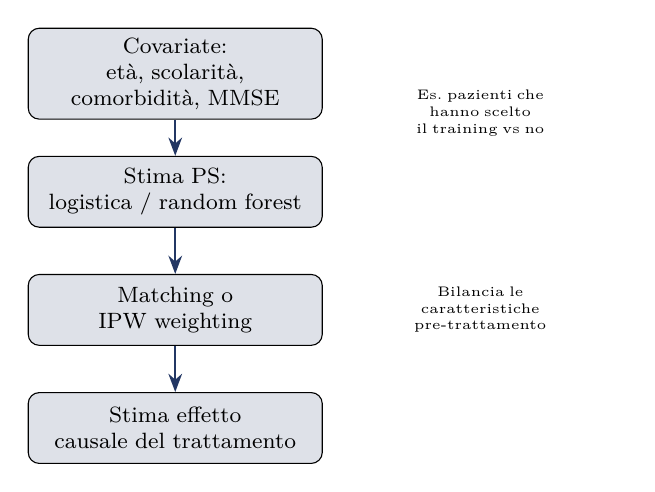
\begin{tikzpicture}[
  box/.style={draw,rounded corners,fill=mblue!15,text width=3.5cm,
              align=center,font=\footnotesize,minimum height=0.9cm},
  arr/.style={-{Stealth},mblue,thick}
]
\node[box] (cov) at (0,4)  {Covariate:\\età, scolarità,\\comorbidità, MMSE};
\node[box] (ps)  at (0,2.5)  {Stima PS:\\logistica / random forest};
\node[box] (mat) at (0,1)  {Matching o\\IPW weighting};
\node[box] (out) at (0,-0.5) {Stima effetto\\causale del trattamento};
\draw[arr] (cov)--(ps); \draw[arr] (ps)--(mat); \draw[arr] (mat)--(out);
\node[right,font=\tiny,text width=3.5cm, align=center] at (2.0,3.5) {Es.\ pazienti che\\ hanno scelto\\il training vs no};
\node[right,font=\tiny,text width=3.5cm, align=center] at (2.0,1) {Bilancia le\\caratteristiche\\ pre-trattamento};
\end{tikzpicture}
\end{center}

\small \textbf{Assunzione chiave (non verificabile!)}:
\emph{no unmeasured confounders}: tutte le variabili che influenzano sia
la selezione al trattamento che l'outcome sono state misurate e incluse
nel PS.
\end{frame}

\begin{frame}{Limiti del Propensity Score}
\phantomsection\label{limiti-del-propensity-score}
\small

\textbf{Assunzione di positività}: ogni soggetto deve avere probabilità
\(> 0\) di ricevere ciascun trattamento. Se alcuni soggetti hanno PS
\(= 0\) o \(= 1\), il confronto non è possibile.

\vspace{0.3em}

\textbf{No unmeasured confounders}: il PS bilancia le covariate
osservate, ma non quelle latenti o non misurate (es.~motivazione del
paziente, supporto familiare non rilevato).

\vspace{0.3em}

\textbf{Overlap insufficiente}: se trattati e controlli sono molto
diversi, il matching non trova coppie adeguate e la stima è poco
affidabile.

\vspace{0.3em}

\textbf{Non è un RCT}: il PS riduce il bias da confounding osservato, ma
non lo elimina completamente. Va sempre affiancato a un'analisi di
sensitività.

\vspace{0.2em}

\tiny Austin (2011). An introduction to propensity score methods.
\emph{Multivariate Behav Res} 46(3). Open Access:
\url{https://doi.org/10.1080/00273171.2011.568786}
\end{frame}

\begin{frame}{Propensity scores e Sensitivity Analysis}
\phantomsection\label{propensity-scores-e-sensitivity-analysis}
Per sondare limiti di PS, spesso vengono utilizzate alcune analisi
aggiuntive di robustezza. Una è la \textbf{Sensitivity Analysis}.

Analisi di E-value (VanderWeele \& Ding, 2017): quantifica quanto forte
dovrebbe essere un confounder non misurato per spiegare l'associazione
osservata.

Più alto è l'E-value, più robusta è l'analisi con Propensity Scores

\vspace{0.2em}

\tiny VanderWeele \& Ding (2017). Sensitivity analysis in observational
research: introducing the E-value. \emph{Ann Intern Med}. Open Access:
\url{https://doi.org/10.7326/M16-2607}
\end{frame}

\begin{frame}{Do-Calculus e Framework di Pearl}
\phantomsection\label{do-calculus-e-framework-di-pearl}
\small

Judea Pearl ha sviluppato un framework basato sui DAG e sul
\textbf{do-calculus} per rispondere a domande causali.

\vspace{0.3em}

\textbf{Differenza fondamentale}:

\begin{itemize}\footnotesize
\item $P(Y \mid X=x)$: probabilità osservata di $Y$ dato che osserviamo $X=x$ (statistica)
\item $P(Y \mid do(X=x))$: probabilità di $Y$ se \emph{interveniamo} impostando $X=x$ (causale)
\end{itemize}

\vspace{0.3em}

\textbf{Backdoor criterion}: un insieme di variabili \(Z\) blocca tutti
i percorsi ``backdoor'' tra trattamento e outcome \(\Rightarrow\)
controllando per \(Z\) si ottiene una stima causale.

\vspace{0.3em}

\textbf{Strumento pratico}: \textbf{DAGitty} (\url{www.dagitty.net})
permette di disegnare DAG online e identificare automaticamente il
minimal adjustment set.

\vspace{0.2em}

\tiny Pearl (2009). \emph{Causality}. Cambridge University
Press.\textbackslash{} Gratis: Pearl et al.~(2016).
\emph{Causal Inference in Statistics: A Primer}. Wiley. Capitoli
disponibili Open Access: \url{http://bayes.cs.ucla.edu/PRIMER/}
\end{frame}

\begin{frame}{Backdoor Criterion: Esempio}
\phantomsection\label{backdoor-criterion-esempio}
\begin{center}
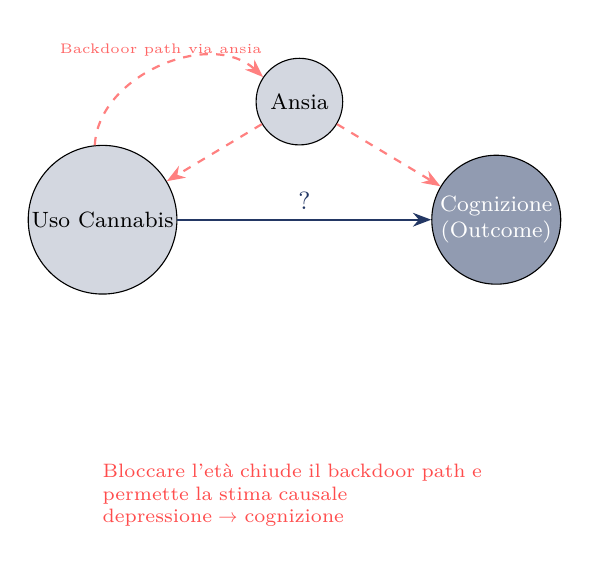
\begin{tikzpicture}[
  node/.style={circle,draw,fill=mblue!20,font=\footnotesize,
               minimum size=1.1cm,inner sep=1pt,align=center},
  blocked/.style={circle,draw,fill=mblue!50,text=white,font=\footnotesize,
                  minimum size=1.1cm,inner sep=1pt,align=center},
  arr/.style={-{Stealth},mblue,thick},
  back/.style={-{Stealth},red!50,dashed,thick}
]
\node[node]    (ansia) at (0,3.5)   {Ansia};
\node[node]    (cann) at (-2.5,2)  {Uso Cannabis};
\node[blocked] (cog) at (2.5,2)   {Cognizione\\(Outcome)};

\draw[arr] (cann)--(cog) node[midway,above,font=\small]{?};
\draw[back] (ansia)--(cog);
\draw[back] (ansia)--(cann);
\draw[back] (cann) to[bend left=65] node[above,font=\tiny,red!60]{Backdoor path via ansia} (ansia);

\node[font=\scriptsize,red!70,text width=5cm] at (0,-1.5)
  {Bloccare l'età chiude il backdoor path e permette la stima causale\\ depressione $\to$ cognizione};
\end{tikzpicture}
\end{center}
\end{frame}

\begin{frame}{Confusion Index: Riepilogo delle Strutture}
\phantomsection\label{confusion-index-riepilogo-delle-strutture}
\begin{center}
\begin{tabular}{>{\footnotesize}l >{\footnotesize}l >{\footnotesize}p{4cm}}
\toprule
\textbf{Struttura} & \textbf{Controllare?} & \textbf{Effetto se si controlla} \\
\midrule
Confounder (fork)  & \textbf{Sì}  & Rimuove associazione spuria \\
Mediatore (chain)  & \textbf{No}  & Blocca parte dell'effetto causale \\
Collider           & \textbf{No}  & Apre un percorso spurio \\
\midrule
\multicolumn{3}{l}{\footnotesize \emph{NB: la scelta dipende dalla domanda causale, non dalla significatività statistica}} \\
\bottomrule
\end{tabular}
\end{center}
\vspace{0.5em}

\small

\includegraphics[width=0.1\linewidth,height=\textheight,keepaspectratio]{Figures/triangle.png}
In psicologia e neuropsicologia, inserire variabili di controllo
``perché correlate'' senza un DAG può produrre stime peggiori di quelle
senza alcun controllo.
\end{frame}

\begin{frame}{Riepilogo: Dalla Correlazione alla Causalità}
\phantomsection\label{riepilogo-dalla-correlazione-alla-causalituxe0}
\begin{center}
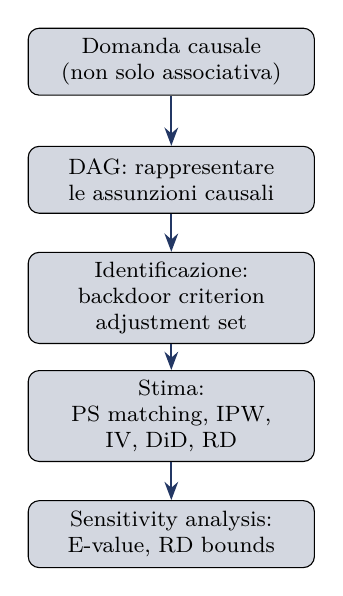
\begin{tikzpicture}[
  box/.style={draw,rounded corners,fill=mblue!20,text width=3.4cm,
              align=center,font=\footnotesize,minimum height=0.85cm},
  arr/.style={-{Stealth},mblue,thick}
]
\node[box] (q)  at (0,4) {Domanda causale\\(non solo associativa)};
\node[box] (dag) at (0,2.5) {DAG: rappresentare\\le assunzioni causali};
\node[box] (id) at (0,1)  {Identificazione:\\backdoor criterion\\adjustment set};
\node[box] (est) at (0,-0.5) {Stima:\\PS matching, IPW,\\IV, DiD, RD};
\node[box] (sen) at (0,-2){Sensitivity analysis:\\E-value, RD bounds};
\draw[arr] (q)--(dag); \draw[arr] (dag)--(id);
\draw[arr] (id)--(est); \draw[arr] (est)--(sen);
\end{tikzpicture}
\end{center}
\end{frame}

\begin{frame}{Come risolvere? Con modelli appropriati.}
\phantomsection\label{come-risolvere-con-modelli-appropriati.}
Tra i modelli appropriati alcuni sono gli \textbf{Structural Equation
Models} (SEM) che:

\begin{itemize}
\tightlist
\item
  modellano esplicitamente direzioni causali.
\item
  tengono conto di errore di misurazioni e possono modellare variabili
  latenti (e.g., Costrutti) con diversi indicatori (e.g., test)
\end{itemize}

NOTA: Ogni SEM è implicitamente un DAG
\end{frame}

\begin{frame}{Cosa NON possono fare i SEM}
\phantomsection\label{cosa-non-possono-fare-i-sem}
\textbf{I SEM non possono}:

\begin{itemize}
\item
  \textbf{dirci la direzione di una causalità} (dobbiamo essere noi a
  ipotizzarla, un modello SEM con direzione completamente sbagliata può
  dare risultati molto forti)
\item
  \textbf{risolvere problemi di campionamento} influenzeranno comunque i
  risultati.
\end{itemize}

-\textbf{dare stime generalizzabili se campione è piccolo} i SEM
rischiano overfitting se il campione non ha grandezza adeguata.
\end{frame}

\begin{frame}{E quindi?}
\phantomsection\label{e-quindi}
Posso fare uno studio con semplici correlazioni o una regressione
multipla e fare quantomeno delle ipotesi?

Sì, può essere utile ma\ldots{} \pause

\begin{center}
\includegraphics[width=0.8\linewidth,height=\textheight,keepaspectratio]{Figures/Lewer_et_al_2025.png}
\end{center}
\centering
\href{https://bmjmedicine.bmj.com/content/4/1/e001375}{\underline{\textbf{Link to OA article}}}
\end{frame}

\begin{frame}{Take-home message}
\phantomsection\label{take-home-message}
Gli studi correlazionali possono sembrare semplici, ma talvolta portano
a conclusioni fuorvianti.

Anche in questo caso, ricordate di interpretare i risultati con giudizio
e alle insidie di interpretare relazioni causa-effetto laddove
potrebbero non esserci.
\end{frame}




\end{document}
